\chapter{初めてのC++、初めてのFK}
\section{プロジェクト作成とビルド} \label{sec:01-proj}
\subsection{プロジェクトの作り方} \label{sec:01-projmake}
\begin{enumerate}
 \item Visual Studio 2013 (以下「VS」)を起動する。
 \item ~ [ファイル]→[新しいプロジェクト]
 \item 表示されたダイアログ左側のツリーメニューで
	[インストール済み]→[テンプレート]→[Visual C++]→[FK]を選択。
 \item 名前は「Hello」、「場所」は以下のようにしておく。
\begin{screen}
\begin{verbatim}
  c:\users\User\documents\proj-semi
\end{verbatim}
\end{screen}
 \item 「OK」を押す。
 \item 「main関数のみ」を選択し、「コンソール出力を使う」にチェックを入れる。
 \item 「完了」を押す。
\end{enumerate}
\subsection{ソースプログラムの編集} \label{sec:01-sourceedit}
VS画面の右側にある「ソリューションエクスプローラー」の中にある、
「main.cpp」をダブルクリックする。すると、main.cpp というファイルを
編集する状態となる。この状態で、以下のようなプログラムを入力してみよう。
\begin{itembox}[l]{最初のプログラム}
\begin{verbatim}
 1: #include <iostream>
 2: 
 3: using namespace std;
 4: 
 5: int main(int, char **)
 6: {
 7:     cout << "Hello World" << endl;
 8:     return 0;
 9: }
\end{verbatim}
\end{itembox}
\subsection{ビルドと実行} \label{sec:01-buildrun}
書いたプログラムは、まずはPCが実行可能な状態に「翻訳」する必要がある。
これを「コンパイル」または「ビルド」と呼ぶ。ビルドするには、
[ビルド]→[ソリューションのビルド]を選択する。
うまく行った場合は「正常終了」という文字の左側が1になっているが、
失敗すると「失敗」という文字の左側が1になっている。
正常終了となるまで修正を繰り返していく必要がある。

実行は、[デバッグ]→[デバッグなしで開始]を選択する。
\section{最も簡単な3Dプログラム} \label{sec:01-start3d}
改めて、新たなプロジェクトを作成する。プロジェクト名はなんでもよいが、
日本語やスペースは避けること。作成したら以下のプログラムを入力してビルドする。\\
~
\begin{itembox}[l]{ウィンドウの表示}
\begin{verbatim}
 1: #include <FK/FK.h>
 2: 
 3: int main(int, char **)
 4: {
 5:     fk_AppWindow window;
 6: 
 7:     window.setSize(800, 600);
 8:     window.setBGColor(0.3, 0.6, 0.8);
 9:     window.open();
10: 
11:     while(window.update() == true) {
12:     }
13: 
14:     return 0;
15: }
\end{verbatim}
\end{itembox}
\subsection*{解説}
\begin{itemize}
 \item 1行目から4行目までは詳細は解説しませんが、
	当面この部分は「最初に書いておくべき呪文」と思ってください。

 \item C++のプログラムでは、「変数」と呼ばれるものを多く用います。
	変数は、主に
	\begin{itemize}
	 \item なんらかの情報を記録するためのもの
	 \item 特定の働きを命令するための道具
	\end{itemize}
	として扱われます。各変数は必ず何らかの「型」を持ちます。
	5行目は、「fk\_AppWindow」という型である
	「window」という変数を用意しているところです。
	このように、C++では「型名 変数名」という単位で変数を準備します。

 \item 基本的に、C++のプログラムは行毎に一つの指示を書いていきますが、
	命令の区切りは「\verb+;+(セミコロン)」です。

 \item 7行目は、window変数を通して「setSize」という\textbf{関数}を用いて、
	ウィンドウのサイズを指定しています。このように、
	\begin{center}
	「\verb+変数名 . 関数名(引数1, 引数2, ...);+」
	\end{center}
	という形式で様々な指示を記述していきます。
	\textbf{引数}というのは、関数に対して入力になる値のことです。
	今回の場合、1番目の引数がウィンドウの横幅、2番目が縦幅を表します。
	setSize関数は fk\_AppWindow 型に備わっている機能です。

 \item 8行目は、ウィンドウの背景色を指定しています。
	光の三原色である赤、緑、青の強さを、最大値が1, 最小値が0 で
	指定します。

 \item 9行目は、これまで指定した指示に従って実際にウィンドウを開く命令です。

 \item 11〜12行目は、書いておかないといきなりウィンドウが消えてしまうのですが、
	現在はそれ以上の意味はありません。
	アニメーションをプログラムするときに、この中身を記述していきます。

 \item 14行目の「\verb+return 0;+」は、プログラムを終了する命令です。
	最後は数字の「ゼロ」であり、アルファベットの「オー」では
	ありませんので注意してください。

\end{itemize}
\newpage
\begin{itembox}[l]{箱の追加}
\begin{verbatim}
 1: #include <FK/FK.h>
 2: 
 3: int main(int, char **)
 4: {
 5:     fk_AppWindow    window;
 6: 
 7:     window.setSize(800, 600);
 8:     window.setBGColor(0.3, 0.6, 0.8);
 9:     window.open();
10: 
11:     fk_Block    block(10.0, 10.0, 10.0);
12:     fk_Model    model1;
13:     model1.setShape(&block);
14:     model1.setMaterial(Yellow);
15:     window.entry(&model1);
16: 
17:     while(window.update() == true) {
18:     }
19: 
20:     return 0;
21: }
\end{verbatim}
\end{itembox}
\subsection*{解説}
\begin{itemize}
 \item 11行目は、新たに「fk\_Block」という型の変数「block」を準備しています。
	これは直方体を生成するための型です。
	ここは window と違って変数名の後に括弧で3つの引数が羅列されています。
	このように、変数名の後に引数を入力することもあります。
	ここでの引数の意味はそれぞれ\(x, y, z\)方向の大きさです。

 \item 12行目の「fk\_Model」は、FKの中で重要な概念となる「モデル」を
	作成するための型なのですが、詳細は次回以降に行います。
	ここでは、「物体を表示するために必要なもの」としておきます。
	13行目で、このモデルの形状が 11 行目で準備した物体であるように
	設定を行っています。14行目では、物体の色が黄色(Yellow)となるように
	設定しています。15行目は、このモデルを実際に表示するものとして
	ウィンドウにエントリー(entry)しています。

\end{itemize}

\section{複数オブジェクトの表示} \label{sec:01-pluralobj}
\begin{itembox}[l]{複数オブジェクトの表示}
\begin{verbatim}
 1: #include <FK/FK.h>
 2: 
 3: int main(int, char **)
 4: {
 5:     fk_AppWindow    window;
 6: 
 7:     window.setSize(800, 600);
 8:     window.setBGColor(0.3, 0.6, 0.8);
 9:     window.open();
10: 
11:     fk_Block    block(10.0, 10.0, 10.0);
12:     fk_Model    model1;
13:     model1.setShape(&block);
14:     model1.setMaterial(Yellow);
15:     window.entry(&model1);
16: 
17:     fk_Sphere   sphere(8, 5.0);
18:     fk_Model    model2;
19:     model2.setShape(&sphere);
20:     model2.setMaterial(Red);
21:     model2.glMoveTo(20.0, 10.0, 0.0);
22:     window.entry(&model2);
23: 
24:     while(window.update() == true) {
25:     }
26: 
27:     return 0;
28: }
\end{verbatim}
\end{itembox}
\subsubsection*{解説}
\begin{itemize}
 \item 17行目の「fk\_Sphere」は球を生成するための型です。
	この変数での引数は、1番目が分割数、2番目が半径を表します。
	分割数は、大きければ大きいほど細かくリアルになっていきますが、
	表示は遅くなっていきます。

 \item 18行目で新たな fk\_Model 型の変数「model2」を準備しています。
	FKでは、複数のモデルを表示する場合にはその個数のモデルを
	準備しておく必要があります。23行目でエントリーを行っていますが、
	これと 15 行目により、
	model1 と model2 の両方が同時に表示されることになります。

 \item 21行目の「glMoveTo」関数は、モデルを平行移動する関数です。
	従って、この球は\((20, 10, 0)\)の位置に移動することになります。

\end{itemize}

\section{物体の向きの制御} \label{sec:01-vec}

\begin{itembox}[l]{箱の向きを変更する}
\begin{verbatim}
 1: #include <FK/FK.h>
 2: 
 3: int main(int, char **)
 4: {
 5:     fk_AppWindow    window;
 6: 
 7:     window.setSize(800, 600);
 8:     window.setBGColor(0.3, 0.6, 0.8);
 9:     window.open();
10: 
11:     fk_Block    block(10.0, 10.0, 10.0);
12:     fk_Model    model1;
13:     model1.setShape(&block);
14:     model1.setMaterial(Yellow);
15:     model1.glVec(1.0, 1.0, 0.0);
16:     model1.glMoveTo(-20.0, -20.0, 0.0);
17:     window.entry(&model1);
18: 
19:     fk_Sphere   sphere(8, 5.0);
20:     fk_Model    model2;
21:     model2.setShape(&sphere);
22:     model2.setMaterial(Red);
23:     window.entry(&model2);
24: 
25:     while(window.update() == true) {
26:     }
27: 
28:     return 0;
29: }
\end{verbatim}
\end{itembox}
\subsubsection*{解説}
\begin{itemize}
 \item 15行目の「glVec」関数は、モデルの向いている方向を変更する関数です。
	今回の場合は\((1, 1, 0)\)の方向に向かせることにより、
	結果的に直方体が斜めを向くかたちになります。
	ちなみに、モデルは初期状態として\(-z\)方向を向いています。
	長細い棒を作成した上で、その棒の向きをベクトルで指定したい場合は、
	\(z\)方向に長い直方体を生成しておく必要があります。
\end{itemize}

\section{練習課題} \label{sec:01-q}
\begin{description}
 \myitem 箱を5個並んだ様子を描画せよ。
 \myitem 白と黒の球が交互に並ぶように配置せよ。
	(色を変更するには setMaterial関数で白は「White」、
	黒は「GlossBlack」を指定する。)
 \myitem 串(Brown)に刺さった三色団子(Red、White、Green)を作成せよ。
 \myitem 串がわずかに斜めに傾いた三色団子を作成せよ。
\end{description}
\begin{figure}[H]
\centering
\includegraphics[scale=0.5]{./Fig/Fig01-01.eps}
\end{figure}
